\documentclass[a4paper,11pt,exos]{nsi} % COMPILE WITH DRAFT
\usepackage{pifont}
\usepackage{fontawesome5}
\usepackage{hyperref}



\begin{document}
\classe{\premiere spe}
\titre{Paradoxe de Braess}
\maketitle

\dleft{12cm}{
    On étudie le réseau routier ABCD représenté ci-contre. Les usagers se déplacent du point A vers le point D et peuvent choisir un des trois itinéraires ABD, ACD ou ABCD.\\ 
    Sur chacune route, le temps de trajet dépend de différents paramètres : le nombre d’usagers circulant sur la route, le nombre de voies disponibles, le nombre de feux rouges, etc ….
}
{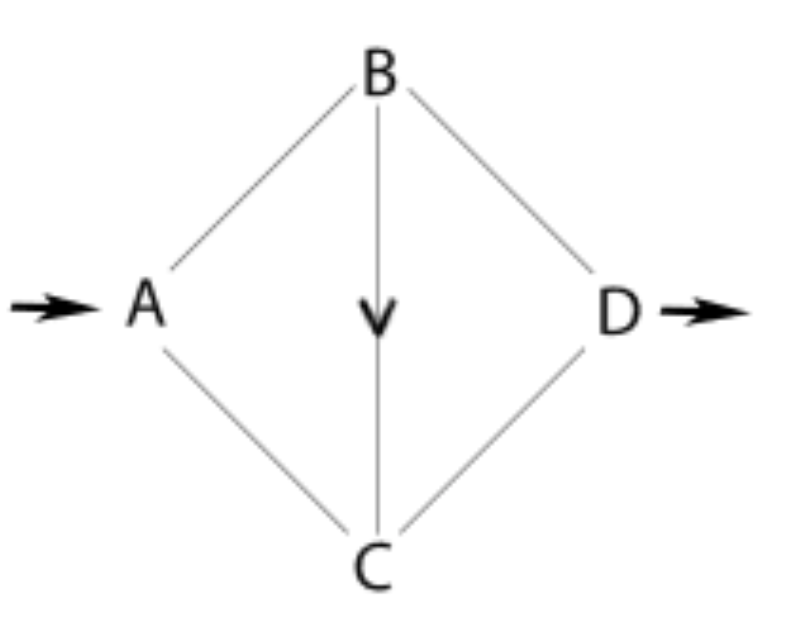
\includegraphics[width=4.5cm]{Braess.png}}

On souhaite étudier la façon dont les usagers vont se répartir sur ce réseau.\\

Pour simplifer notre modèle, on suppose que le temps de trajet sur une route dépend de la proportion des usagers l’empruntant, de manière constante ou polynomiale de degré 1 ou 2.\\
On modélise les temps de trajet sur les routes du réseau par les fonctions suivantes : 
\begin{enumerate}[label=\textbullet]
    \item $f_{AB}(p)=3+p+16p^2$ où $p$ représente la proportion d’usagers circulant sur la route AB ;
    \item $f_{BD}(p)=10+2p$ où $p$ représente la proportion d’usagers circulant sur la route BD ;
    \item $f_{AC}(p)=22$ où $p$ représente la proportion d’usagers circulant sur la route AC ;
    \item $f_{CD}(p)=2+3,5p+3p^2$ où $p$ représente la proportion d’usagers circulant sur la route CD ;
    \item $f_{BC}(p)=0,5$ où $p$ représente la proportion d’usagers circulant sur la route BC.
\end{enumerate}

\textbf{Les temps de trajet sont exprimées en minutes.} \textit{Si nécessaire, vous arrondirez vos résultats à l’unité.}

\subsection*{Partie 1 : Comprendre et interpréter le modèle}

Étudions un premier exemple :\\
Supposons que 20 \% des usagers circulent sur la route BD.\\
On a donc $p=0,2$ et $f_{BD}(0,2)=10+2\times0,2=10,4$.\\
Le temps de trajet sur la route BD est donc de $10,4$ minutes soit $10$ minutes et $0,4\times 60= 24$ secondes.

\begin{enumerate}
    \item Calculer $f_{AB}(0)$. Interpréter ce résultat dans le contexte de l’exercice.\\[.5em]
    \carreauxseyes{16}{2.4}
    \item Calculer $f_{AB}(1)$. Interpréter ce résultat dans le contexte de l’exercice.\\[.5em]
    \carreauxseyes{16}{2.4}
    \item Calculer $f_{AB}(0,5)$. Interpréter ce résultat dans le contexte de l’exercice.\\[.5em]
    \carreauxseyes{16}{2.4}
    \item La fonction $f_{AC}$ est une fonction constante. Que peut-on en déduire pour le temps de trajet sur la route AC ?\\[.5em]
    \carreauxseyes{16}{1.6}
\end{enumerate}

\subsection*{Partie 2 : Répartition des usagers sur le réseau}
Pour aller de A vers D, les usagers peuvent choisir un des 3 itinéraires : ABD, ABCD et ACD. Les usagers vont
choisir l’itinéraire qui sera le plus rapide pour eux. Ce temps varie en fonction de l’affluence sur le réseau modélisé par la variable $p$.

\begin{enumerate}
    \item Les itinéraires ABD et ABCD commencent de la même façon : pour les comparer, il suffit donc de comparer les temps de trajet de BD et BCD.
    \begin{enumalph}
        \item Quel est le sens de variation de la fonction $f_{BD}$ sur l'intervalle $\fif{0}{1}$ ?\\[.5em]
        \carreauxseyes{16}{2.4}
        \item On note $f_{BCD}(p)$ le temps de trajet sur l’itinéraire BCD en fonction de la proportion $p$ d'usagers circulant sur BCD. Exprimer $f_{BCD}(p)$ en fonction de $p$.\\
        En déduire le sens de variation de la fonction $f_{BCD}$ sur l'intervalle $\fif{0}{1}$.\\[.5em]
        \carreauxseyes{16}{4}
        \item Compléter les tableaux de variations des fonctions $f_{BD}$ et $f_{BCD}$ sur l'intervalle $\fif{0}{1}$.
        \begin{multicols}{2}
            \begin{center}
                \begin{tikzpicture}
                \tkzTabInit[color,lgt=2.8,espcl=4]
                {$x$/.7,variations de $f_{BD}$ /2}
                {0,1}
                \tkzTabVar{}
                \end{tikzpicture}
            \end{center}
            \begin{center}
                \begin{tikzpicture}
                \tkzTabInit[color,lgt=2.8,espcl=4]
                {$x$/.7,variations de $f_{BCD}$ /2}
                {0,1}
                \tkzTabVar{}
                \end{tikzpicture}
            \end{center}
        \end{multicols}
        \item Comparer les temps de trajet sur les itinéraires BD et BCD. Que vont faire les usagers ?\\[.5em]
        \carreauxseyes{16}{2.4}
    \end{enumalph}
    \item Les itinéraires ACD et ABCD se terminent de la même façon : pour les comparer, il suffit donc de comparer les temps de trajet sur AC et ABC.
    \begin{enumalph}
        \item Quel est le temps de trajet sur la route AC ?\\[.5em]
        \carreauxseyes{16}{1.6}
        \item $f_{ABC}(p)$ est le temps de trajet sur l’itinéraire ABC en fonction de la proportion $p$ d'usagers circulant sur ABC. Exprimer $f_{ABC}(p)$ en fonction de $p$.\\
        En déduire le sens de variation de la fonction $f_{ABC}$ sur l'intervalle $\fif{0}{1}$.\\[.5em]
        \carreauxseyes{16}{4}
        \item Compléter les tableaux de variations des fonctions $f_{AC}$ et $f_{ABC}$ sur l'intervalle $\fif{0}{1}$.
        \begin{multicols}{2}
            \begin{center}
                \begin{tikzpicture}
                \tkzTabInit[color,lgt=2.8,espcl=4]
                {$x$/.7,variations de $f_{AC}$ /2}
                {0,1}
                \tkzTabVar{}
                \end{tikzpicture}
            \end{center}
            \begin{center}
                \begin{tikzpicture}
                \tkzTabInit[color,lgt=2.8,espcl=4]
                {$x$/.7,variations de $f_{ABC}$ /2}
                {0,1}
                \tkzTabVar{}
                \end{tikzpicture}
            \end{center}
        \end{multicols}
        \item Comparer les temps de trajet sur les itinéraires AC et ABC. Que vont faire les usagers ?\\[.5em]
        \carreauxseyes{16}{4}
        \item En déduire l’itinéraire que les usagers vont préférer. Quel est le temps de trajet sur cet itinéraire à l'heure de pointe ?\\[.5em]
        \carreauxseyes{16}{1.6}
    \end{enumalph}
\end{enumerate}
\carreauxseyes{16.8}{4.8}

\subsection*{Partie 2 : Fermeture de la route BC}
\dleft{12cm}{
    Dans le cadre de travaux de rénovation de la voirie, la route BC sera fermée à la circulation pendant toute une année. Les autorités craignent que les conditions de circulation ne se détériorent sur le réseau. Nous nous proposons de reprendre l’étude précédente sur le nouveau réseau.\\

    Dans cette partie, on suppose que c’est l’heure de pointe : 100 \% des usagers sont en circulation sur le réseau et se répartissent sur le réseau. On désigne par $x$ la proportion d’usagers ayant choisi l’itinéraire ABD. 
La proportion d’usagers ayant choisi l’itinéraire ACD est donc $1-x$.
}
{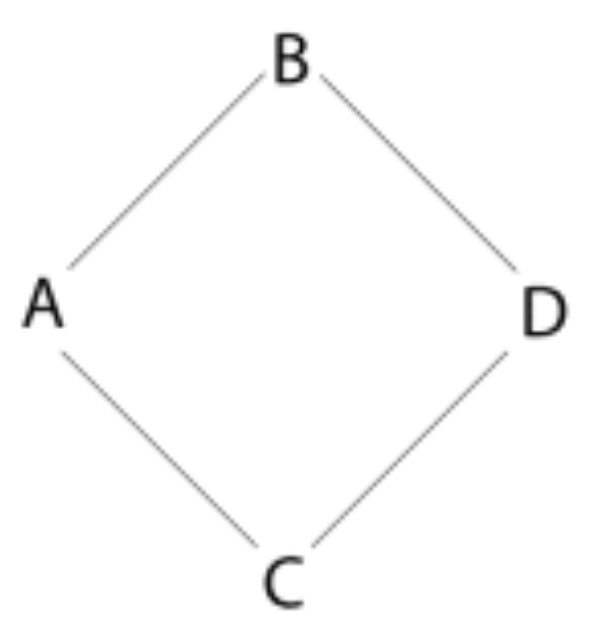
\includegraphics[width=4.5cm]{Braess2.png}}
\begin{enumerate}
    \item Exprimer $T_B(x)$ le temps de trajet des usagers qui ont choisi l’itinéraire ABD en fonction de $x$.\\[.5em]
    \carreauxseyes{16}{3.2}
    \item Montrer que le temps de trajet des usagers qui ont choisi ACD est $T_C(x)=3x^2-9,5x+30,5$.\\[.5em]
    \carreauxseyes{16}{3.2}
    \item Comparer $T_B(0,2)$ et $T_C(0,2)$. Que vont faire les usagers à la prochaine heure de pointe ?\\[.5em]
    \carreauxseyes{16}{4}
    \item \faCalculator \hspace*{0.2cm} Représenter graphiquement les fonctions $T_B$ et $T_C$ sur l’intervalle $\fif{0}{1}$.
    \begin{center}
        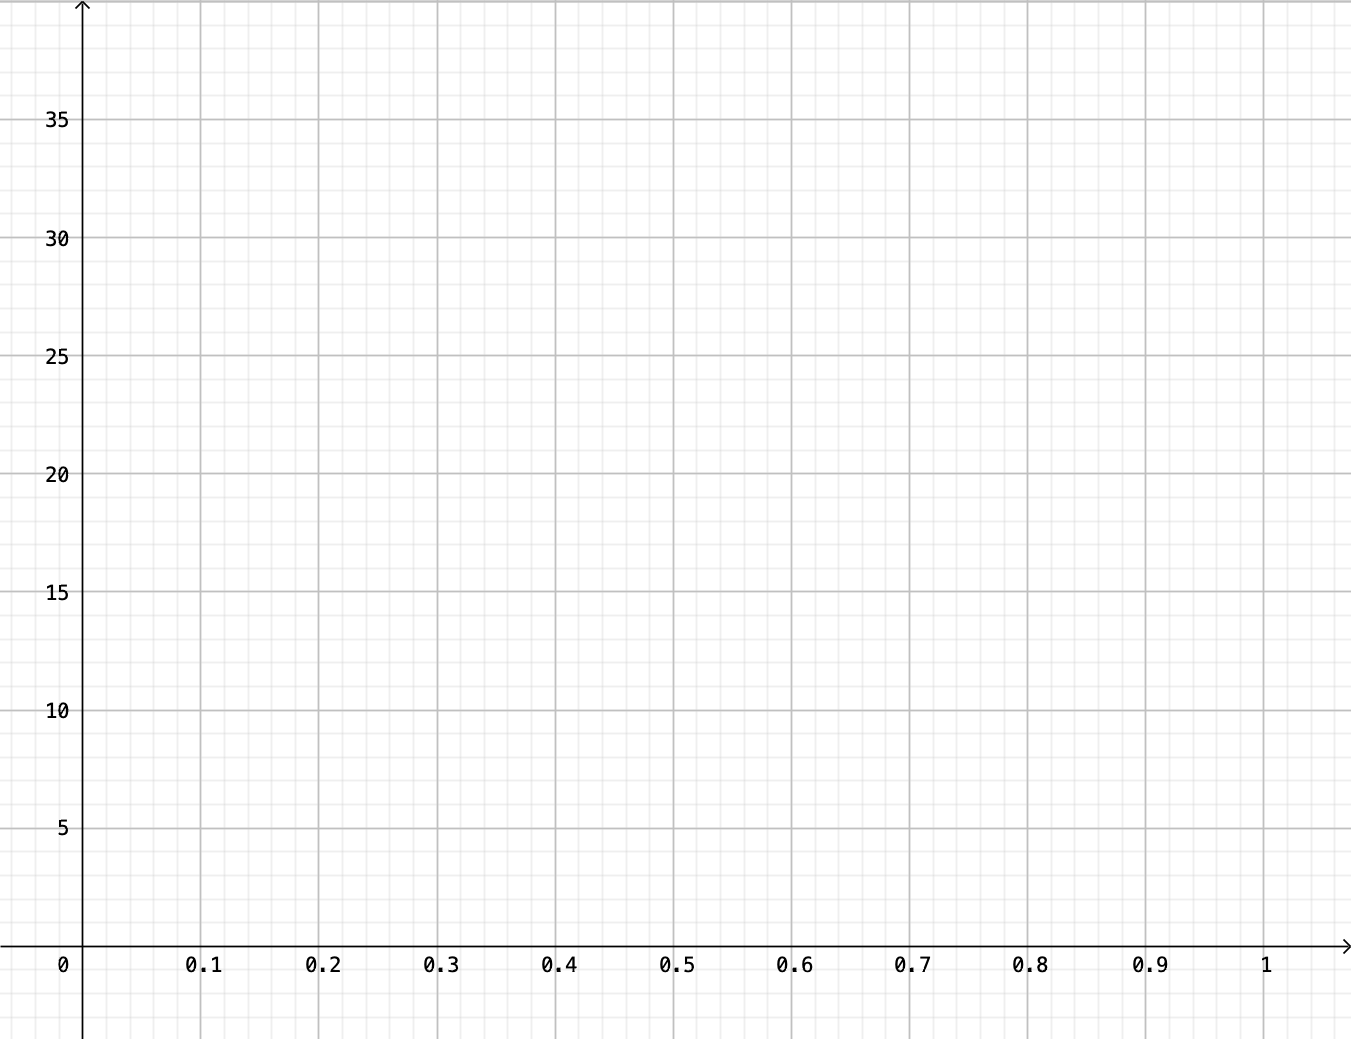
\includegraphics[width=10.5cm]{repere.png}
    \end{center}
    \item L'état d'équilibre du réseau routier étudié correspond à la situation pour laquelle les usagers se sont répartis sur le réseau de telle sorte que les temps de trajet soient les mêmes sur les deux itinéraires. 
    \begin{enumalph}
        \item Calculer l'état d'équilibre du réseau routier. Interpréter cet état dans le contexte de l'activité.\\[.5em]
        \carreauxseyes{16}{8}
        \item Lorsque le réseau est à son équilibre, calculer le temps de trajet pour aller de A vers D. Comparer ce temps avec le temps obtenu à la question \textbf{3.} de la partie 2.\\[.5em]
        \carreauxseyes{16}{4}
    \end{enumalph}
\end{enumerate}
\end{document}